% !TeX root = ../main.tex
% Add the above to each chapter to make compiling the PDF easier in some editors.
\chapter{Time Series Generation Tool}\label{chapter:tool}

We have looked in detail at two approaches of generating time series, first studying their theory, then implementing them in Python. The result of this is a command line tool for generating time series. This chapter will discuss the usage of this tool. \parencite{tsgenerator}

\section{General Options}

There are a lot of command line options available in this tool. We will first go over the general ones. 

"--method": On a high level there are four different modes of operation. Three are based on Hidden Markov Models and one on Singular Spectrum Analysis. They are called "hmm-learn", "hmm-param-simple", "hmm-param", and "ssa". This option selects which one of them to use. 

"--length": All methods are able to generate time-series of variable length. This option specifies how many samples should be generated. 

"--output": The tool will output the time-series in the CSV format. One column will be the time points and the second column will contain the generated values. Using output you can specify a file to write this CSV data to. If none is specified the data will be printed to stdout. 

"--time-increment": This affects the the values in the first "time" column of the output. By default the increment is 1, but it can be changed with this option. 

"--scaling": For this option you specify two values: a new minimum and a new maximum. After generation of your chosen method is complete, this applies scaling so that the minimum and maximum values of the time-series become the specified ones. 

"--display": By default the time series is only output in CSV text form. If this option is enabled the tool will display a graph of the generated series as well. This is very helpful for visualization!

\section{hmm-learn}

The first available method is "hmm-learn". The idea is to specify training time series, from which the tool learns HMM parameters, that are then used to generate the time-series. This method comes with its own options. 

"--hmm-training": This is a path to a CSV containing the training data. Each row is considered one individual time-series. 

"--hmm-components": This is the number of hidden states to use in the HMM. 

"--hmm-iterations": This is the number iterations that the EM-algorithm will be run. This number does not have to be huge since the algorithm usually converges quite quickly. 10 to 50 iterations are a good range. 

"--display": This will print the current iteration number and the current log-likelihood during every iteration. This can be helpful since depending on the setup the learning step can take quite a while. Also by looking at the log-likelihood you can get a sense of the convergence. 

\begin{figure}
\begin{singlespace}
\begin{lstlisting}[language=Python]
def generate_hmm(startprop, transmat, means, cov, l):
    k = startprop.size
    start = np.random.choice(range(k), p=startprop)
    mu = means[start]
    hiddenstates = [start]
    sigma = np.sqrt(cov[start])
    first_output = np.random.normal(mu, sigma)
    samples = [first_output]
    for _ in range(l-1):
        prevstate = hiddenstates[-1]
        nextstate = np.random.choice(range(k), p=transmat[prevstate])
        hiddenstates += [nextstate]
        mu = means[nextstate]
        sigma = np.sqrt(cov[nextstate])
        next_output = np.random.normal(mu, sigma)
        samples += [next_output]
    return samples
\end{lstlisting}
\end{singlespace}
\caption{generate\_hmm function}    
\label{fig:hmm-generate}
\end{figure}

We have looked at the implementation of the parameter learning using the Baum-Welch algorithm in detail. However we have not looked at the actual time-series generation code. The implementation from the tool is listed in Figure \ref{fig:hmm-generate}. 

The idea is to generate a hidden state sequence based on the start and transition probabilities. For this "np.random.choice" from numpy is used, which allows drawing from a set with a given probability vector p. From the hidden states we obtain the corresponding means and variances and draw the data points from a normal distribution using "np.random.normal". 

\section{hmm-param}

This method works by specifying the HMM parameters manually instead of learning them from training data. This method offers the following options: 

"--hmm-means": This is the means $\mu$ parameter in a semi-continuos HMM. 

"--hmm-cov": This is the variance $\sigma$ parameter in a semi-continuos HMM. 

"--hmm-start-prop": This is the start probability parameter $\pi$ in a HMM. 

"--hmm-trans-prop": This is the transition probability parameter $a$ in a HMM. 

Note that the dimensions of these parameters have to match up. "means", "cov", and "start-prop" all need to have the same length k, while "trans-prop" needs to be the square of that: $k^2$. 

\section{hmm-simple-param}

This tool already requires a lot of commandline options to be specified. However in the "hmm-param" method this becomes unreasonable. This is why the "hmm-simple-param" method exists, where you only have to specify the means: 

"--hmm-means": This is the means $\mu$ parameter in a semi-continuos HMM. 

For the rest of the parameters the tool will pick for you. The variance will be 20\% of the covariance of the means vector for every state. The start probabilities will be evenly distributed. The transition probabilities are also evenly distributed, but with a bias towards staying in the same state. 

As an example consider that the following means vector was given: 

\begin{equation}
    \mu = (10, 30, 40, 70)^T
\end{equation}

Then the remaining parameters will be chosen in this way:

\begin{equation}
    \begin{split}
    a = 
    \begin{pmatrix}
        0.625 & 0.125 & 0.125 & 0.125 \\
        0.125 & 0.625 & 0.125 & 0.125 \\
        0.125 & 0.125 & 0.625 & 0.125 \\
        0.125 & 0.125 & 0.125 & 0.625
    \end{pmatrix} \\
    \sigma^2 = (144, 144, 144, 144)^T \\
    \pi = (0.25, 0.25, 0.25, 0.25)^T 
\end{split}
\end{equation}

\section{ssa}

The last method of generating is using Singular Spectrum Analysis forecasting. This also offers some commandline options: 

"--ssa-original": This points towards a CSV file with the time series that is to be forecasted. 

"--ssa-window": This is the window length for the SSA embedding. This should not be to small but also not larger than $N/2$ where N is the length of the original series. If there is seasonality in the data it should be a multiple of that. 

"--ssa-components": This is the number of eigentriple components to use in the time-series approximation and in the recurrence forecasting. Smaller values will lead to a smoother approximation, while large ones make the approximation more accurate. 

\section{Examples}

Figure \ref{fig:hmm-learn-example} shows an example of the usage of the hmm-learn method. The specified training data is a time-series of daily page views of Wikipedia in 2019. (Reference)

Figure \ref{fig:hmm-param-simple-example} show and example of the usage of the hmm-param-simple method. It uses the previously discussed example $\mu = (10, 30, 40, 70)^T$. 

Figure \ref{fig:hmm-param-example} is the exact same parameters as Figure \ref{fig:hmm-param-simple-example}, but with all the parameters spelled out manually using the hmm-param method. 

Figure \ref{fig:ssa-example} is an example of the ssa method. The data is airplane passenger data per month in the US. This is an ideal time-series for SSA since there is a clear trend and seasonality. The original time series is 144 long, so the values past that are all forecasted.

\begin{figure}
\begin{lstlisting}[language=bash]
    python generate.py --method hmm-learn \
    --hmm-training wikipedia-overall-2019-list.csv --hmm-components 4 \
    --hmm-iterations 10 --show-progress --length 20 --display
\end{lstlisting}
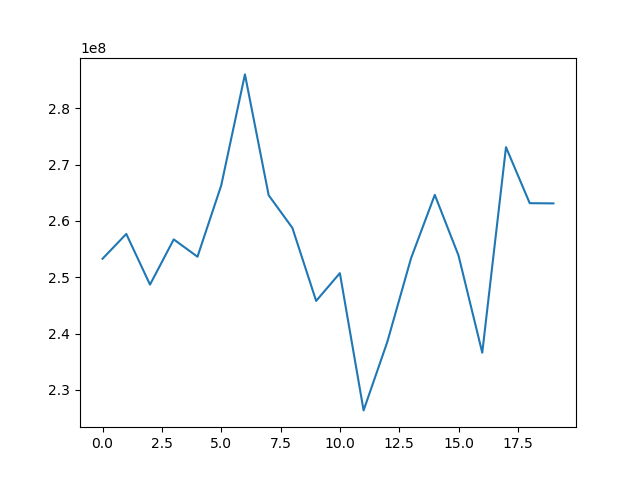
\includegraphics[scale=0.7]{figures/hmm-learn}
\caption{hmm-learn Example}    
\label{fig:hmm-learn-example}
\end{figure}

\begin{figure}
\begin{lstlisting}[language=bash]
    python generate.py --method hmm-param-simple --length 20 \
    --hmm-simple-means 10 30 40 70 --display
\end{lstlisting}
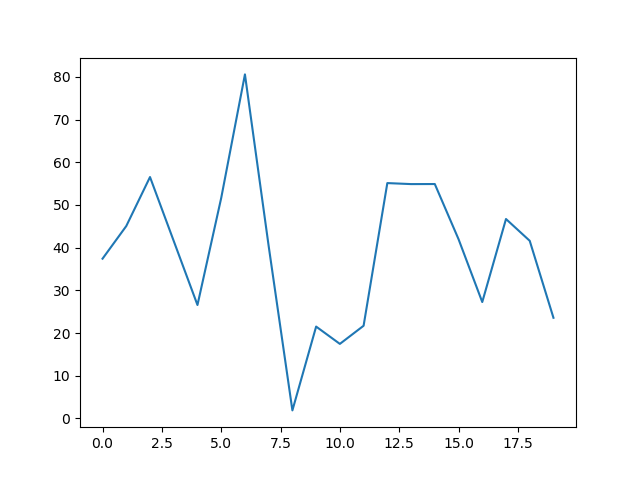
\includegraphics[scale=0.7]{figures/hmm-param-simple}
\caption{hmm-learn Example}    
\label{fig:hmm-param-simple-example}
\end{figure}

\begin{figure}
\begin{lstlisting}[language=bash]
    python generate.py --method hmm-param --length 20 \
    --hmm-means 10 30 40 70 --hmm-cov 144 144 144 144 \
    --hmm-start-prop 0.25 0.25 0.25 0.25 --hmm-trans-prop \
    0.625 0.125 0.125 0.125 0.125 0.625 0.125 0.125 0.125 \
    0.125 0.625 0.125 0.125 0.125 0.125 0.625 --display
\end{lstlisting}
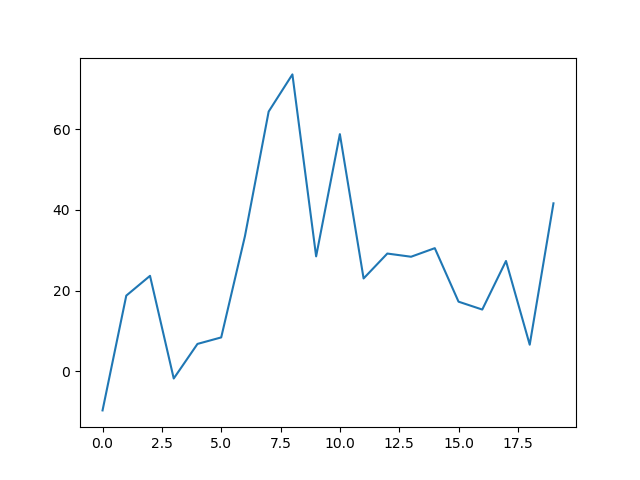
\includegraphics[scale=0.7]{figures/hmm-param}
\caption{hmm-param Example}    
\label{fig:hmm-param-example}
\end{figure}

\begin{figure}
\begin{lstlisting}[language=bash]
    python generate.py --method ssa --length 170 --ssa-original \
    airpassenger-list.csv --ssa-window 36 --ssa-components 13 --display
\end{lstlisting}
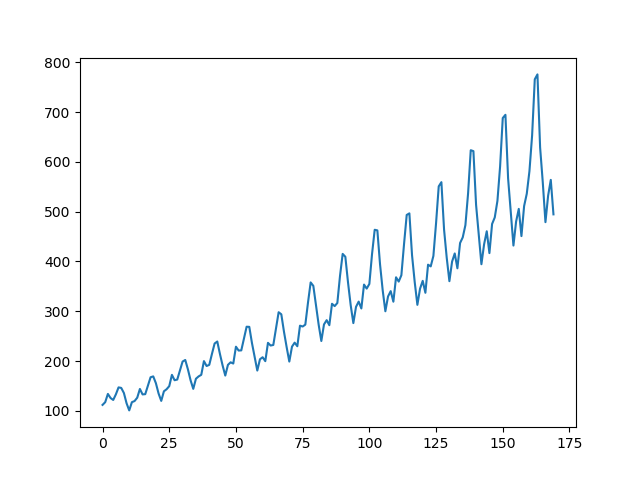
\includegraphics[scale=0.7]{figures/ssa}
\caption{ssa Example}    
\label{fig:ssa-example}
\end{figure}